\chapter{Evaluation}
\label{sec:framework}

With AndroMEDA, we attempt to build on top of the Android Permission system, to do a better job at enforcing the User-App Agreement. The main reasons why the Permission System failed to differentiate between malware and normal software can be seen as a lack of context and understanding of use. When an app requests a permission, it is granted to the app regardless of any context - at any time, and regardless of user consent. The data, after being requested, ultimately can be manipulated and transmitted to any party without user consent. 

Projects like TaintDroid\citep{enck2010taintdroid} have begun to address the flow of personal data, which aids in the user understanding the use of data. However, much more can be done to address both context and use, which AndroMEDA addresses. By instrumenting API calls, AndroMEDA can both inspect context use of personal data as well as other important system actions. By presenting this normally hidden information to the user, AndroMEDA provides them with a feedback loop to evaluate whether the User-App Agreement has been broken.

\section{Existing Malware Datasets}
%To test the effectiveness of AndroMEDA at detecting malicious behavior, we begin with testing apps from the Android Malware Genome Project\citep{zhou2012dissecting}, the most comprehensive academic malware dataset. Unfortunately, we found only 31 (2.4\%) of the nearly 1300 samples were designed for Android 2.3 and above, when Android fixed many rootkits, and not a single one targeted Android 4.0 or above, when Android took steps to fix SMS related malware. Furthermore, we found many of the samples simply did not run anymore, due to deprecated APIs and other poor coding techniques.



To test the effectiveness of AndroMEDA at detecting malicious behavior, we begin with testing apps from the Android Malware Genome Project\citep{zhou2012dissecting}, the most comprehensive academic malware dataset. Unfortunately, as show in in Figure \ref{fig:malwaresdk}, we found only 31 (2.4\%) of the nearly 1300 samples were designed for Android 2.3 and above, when Android fixed many rootkits, and not a single one targeted Android 4.0 or above, when Android took steps to fix SMS related malware. When looking for malware that runs on Android 2.3 and above that do not use a root exploit, we find only 4 samples - 0.3\% - fit. 

\begin{figure}[h]
\begin{center}
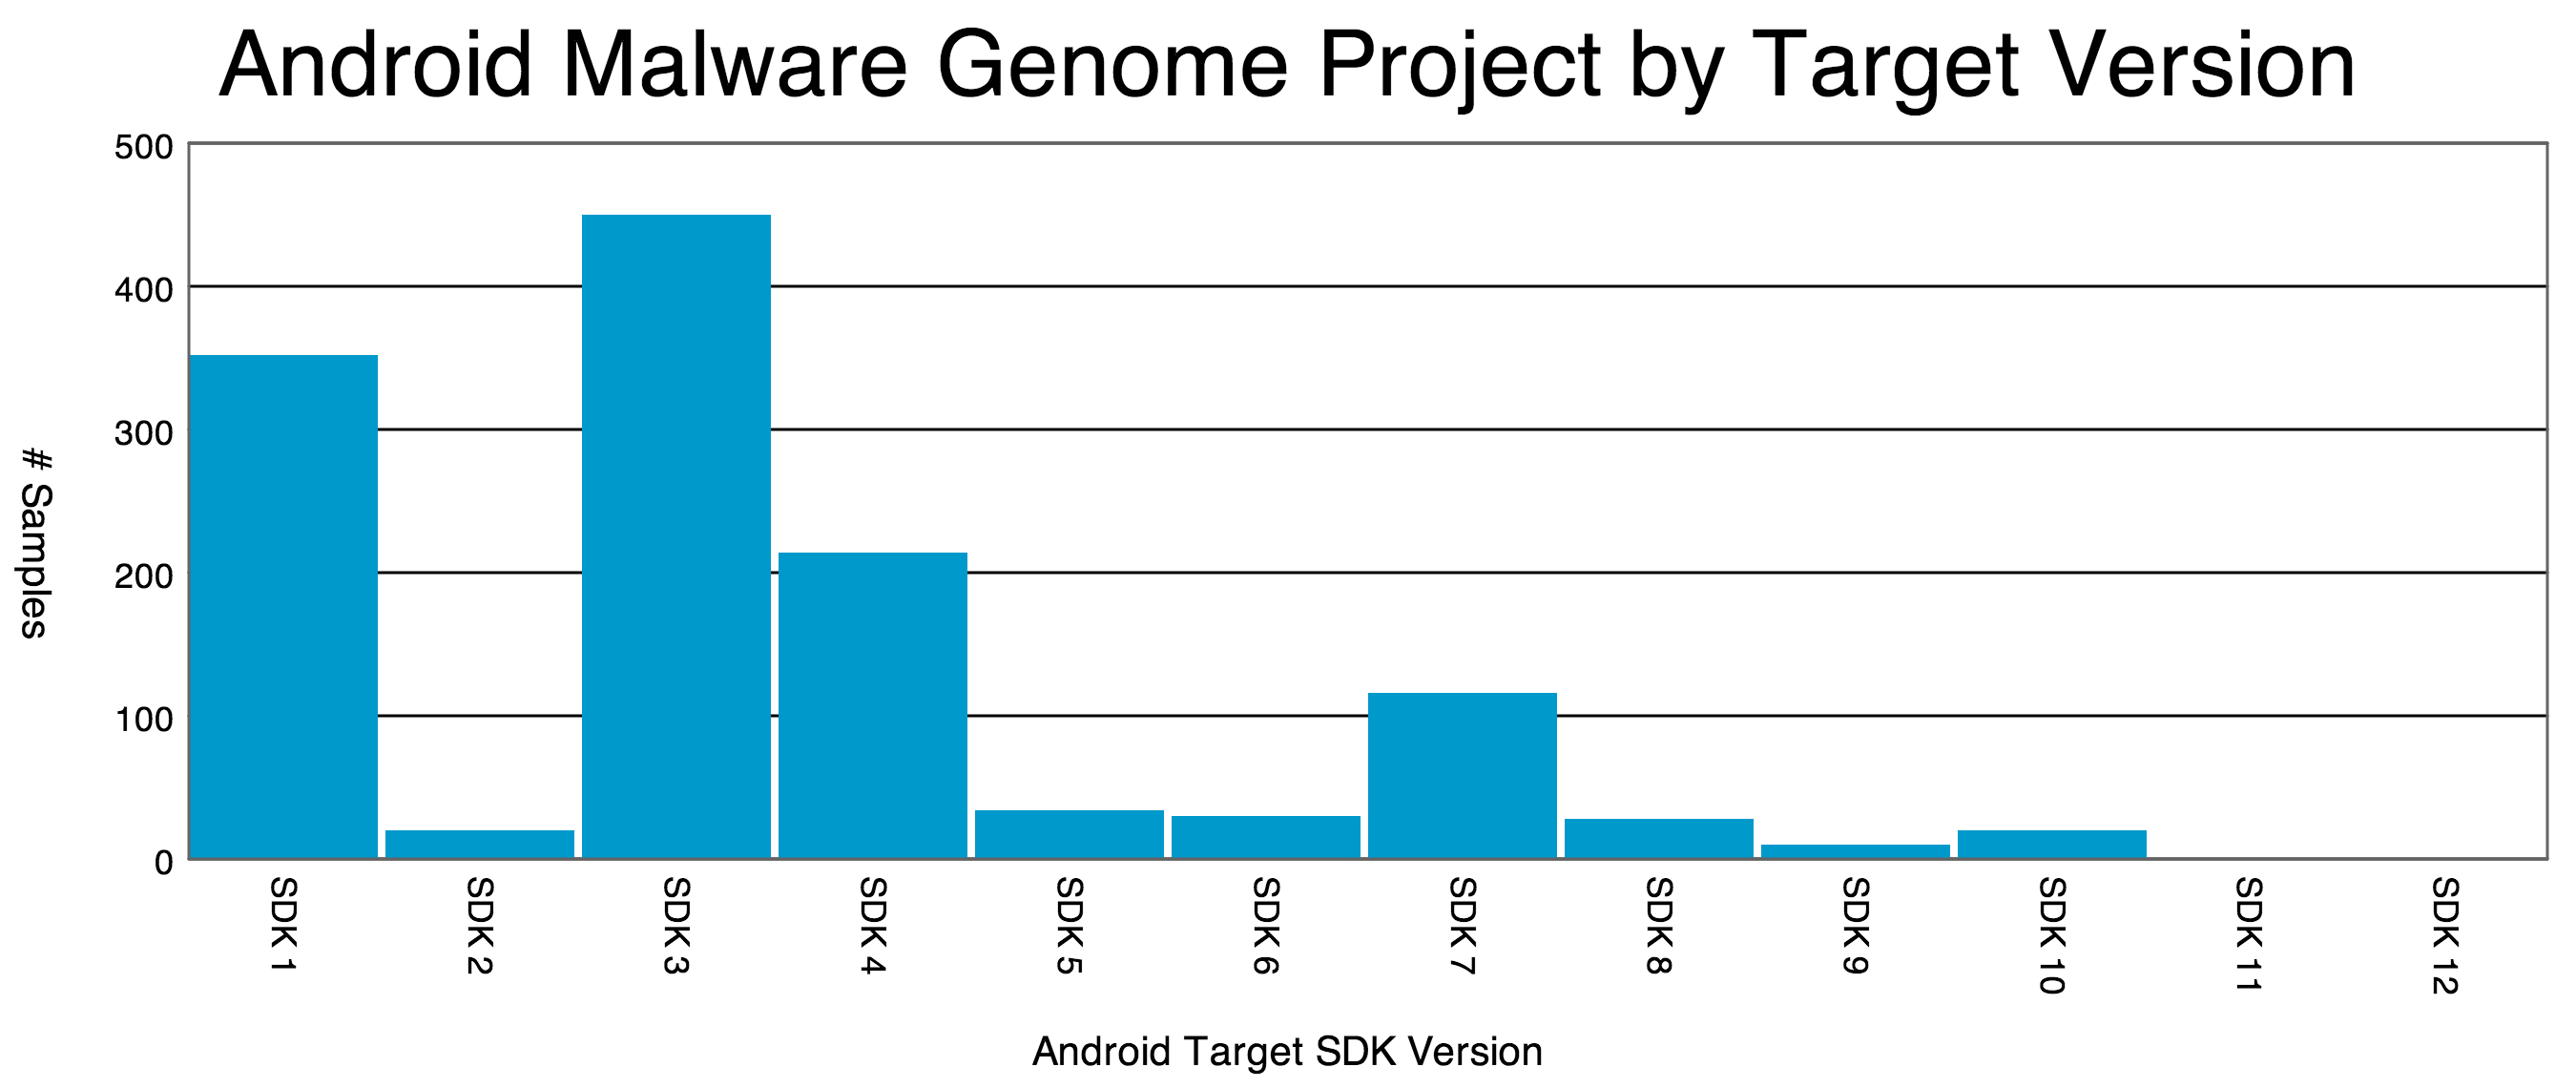
\includegraphics[width=1.0\columnwidth]{figs/MalwareAndSDK}
\caption{Malware from the Android Malware Genome Project by Android Version }
\label{fig:malwaresdk}
\end{center}
\end{figure}

Of these 4 examples, one, \textit{RogueSPPush}, sends premium SMS messages, but does not request \textit{Send SMS}, rendering it ineffective. The 3 remaining samples, \textit{DogWars}, \textit{GoldDream} and \textit{DroidDreamLight} were Info Theft malware. We found \textit{DroidDreamLight} to be less than worthwhile for testing, due to its rather benign nature: the worst action it performs is uploading the device's IMEI to a remote server. Finally, \textit{GoldDream} has botnet capabilities, making it difficult to test, due to the lack of an existing botnet.

The remaining app, \textit{DogWars}, makes a good testing app. Made as a ``hacktivist'' app in protest of an existing app\citep{symantecdogwars}, \textit{DogWars} repackages a game with code to send SMS messages to all contacts on the next boot. The screenshots in Figure \ref{fig:dogwars_visual} show how AndroMEDA clearly identifies when DogWars accesses contacts and sends messages, and allows the user to identify it as malware.

\begin{figure}[h]
\begin{center}
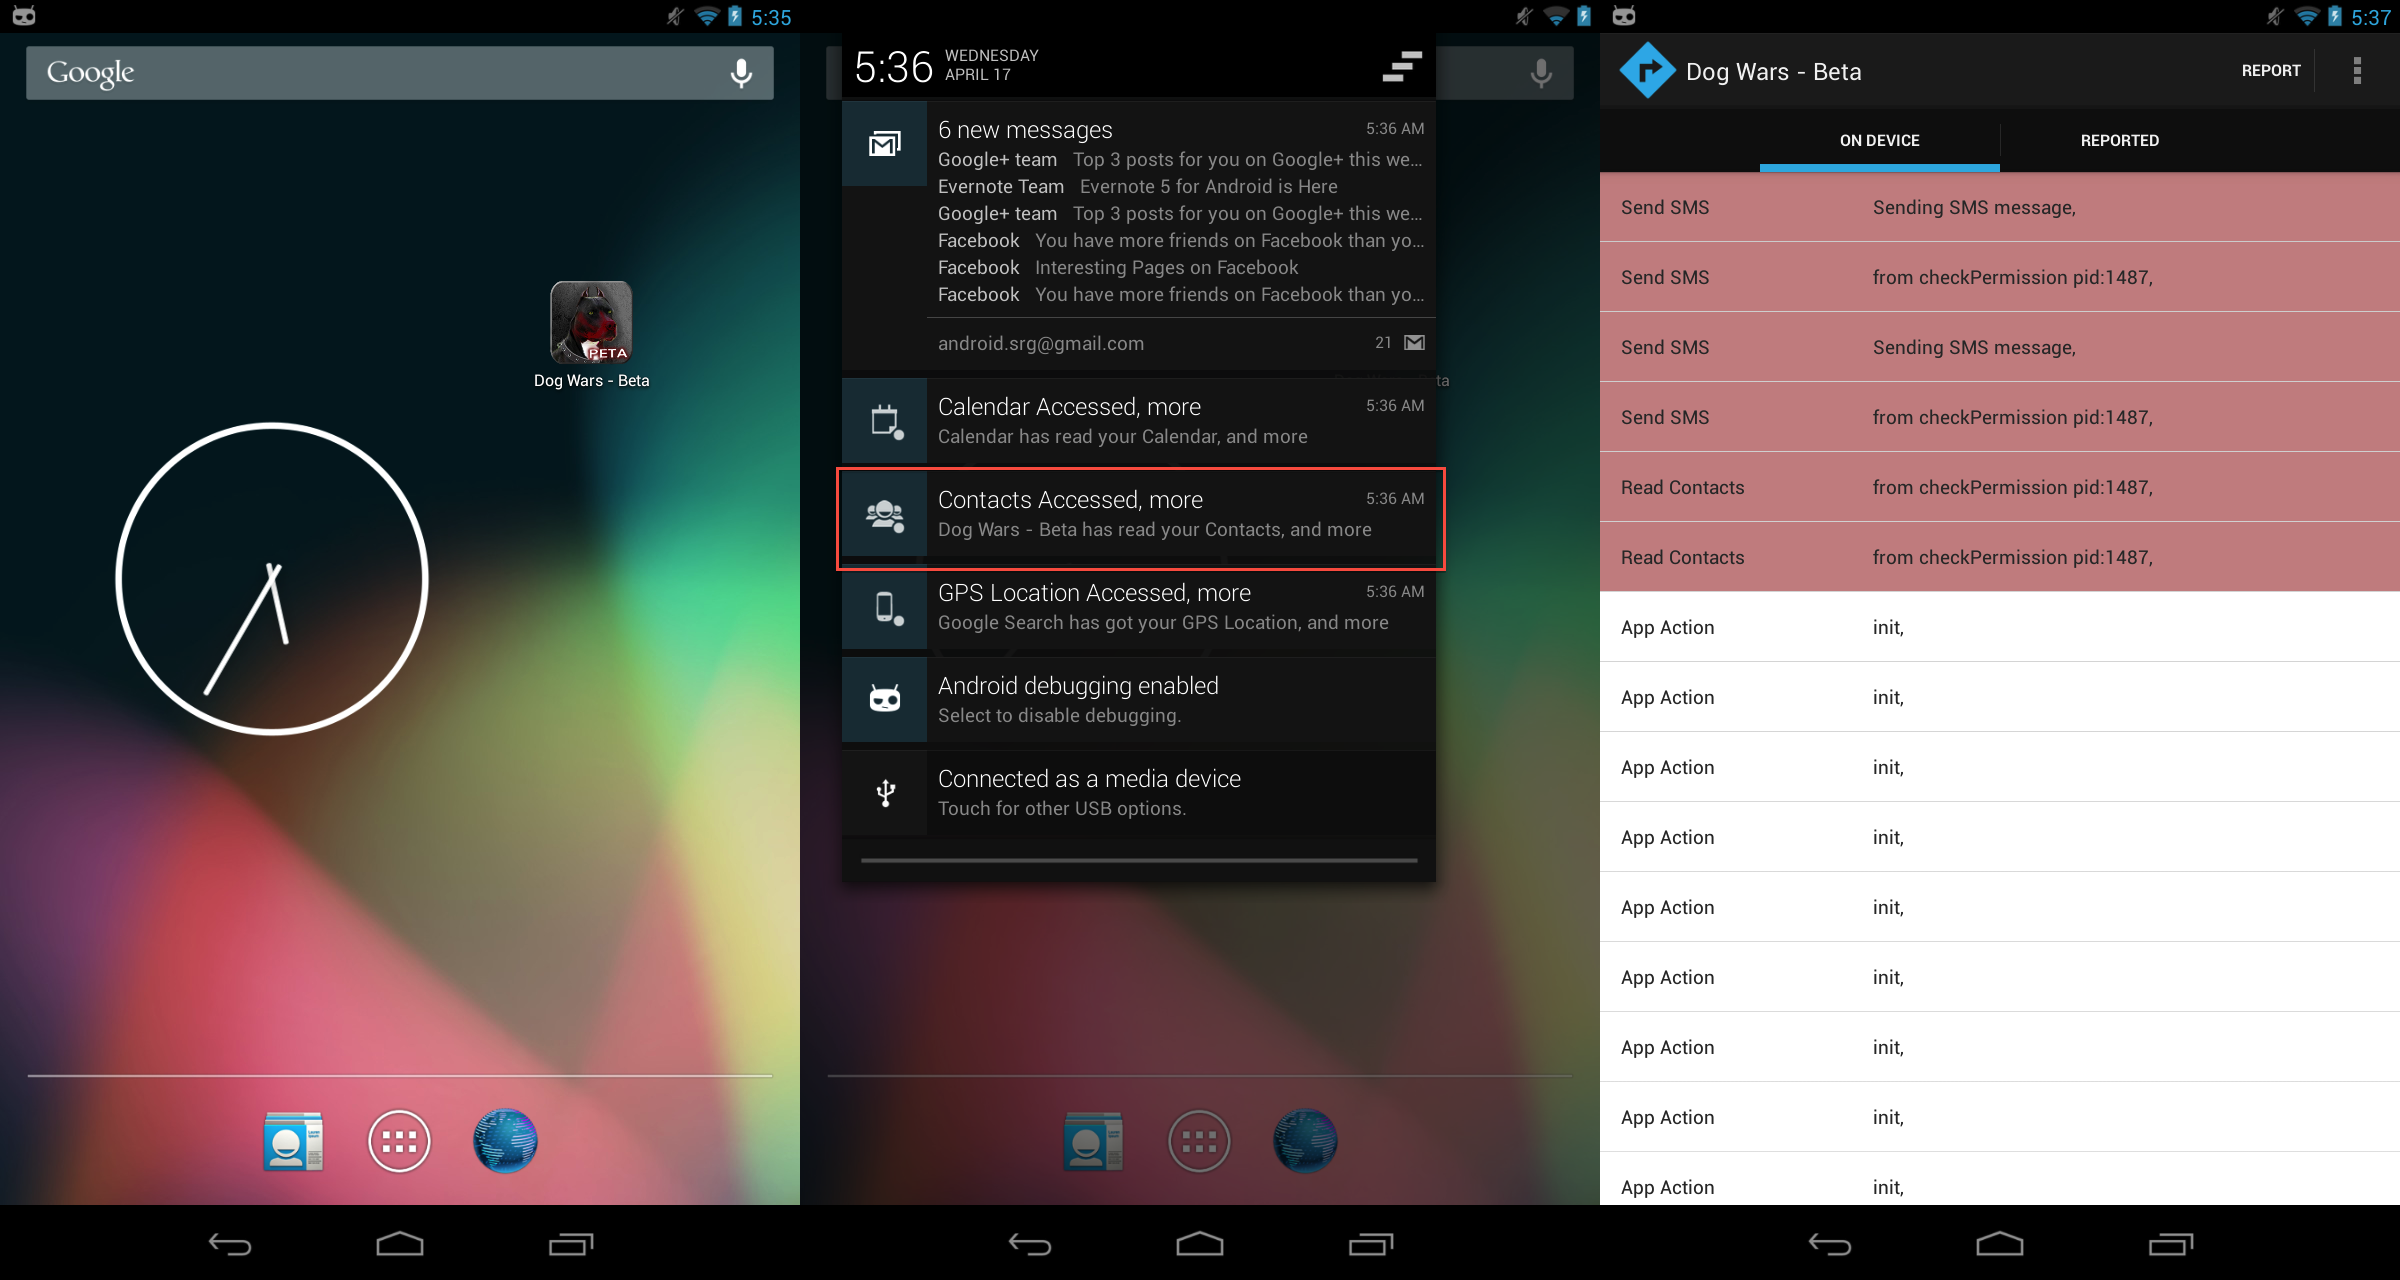
\includegraphics[width=1.0\columnwidth]{figs/dogwars_detection}
\caption{AndroMEDA detecting the \textit{DogWars} Malware (annotated in red) }
\label{fig:dogwars_visual}
\end{center}
\end{figure}

We have demonstrated AndroMEDA's ability to identify malware in existing datasets, but in the process we highlighted the shortcomings of the current Android malware datasets. To test a future-malware oriented framework, it would be ideal to have more sophisticated malware. Rootkits and Premium SMS malware have been addressed by recent versions of Android, so we focus on what we believe to be the future of malware on Android: sophisticated Info Theft Apps. The concept of hiding Info Theft Malware inside of benign apps, designed to silently steal PII and perform other unwanted operations, we have dubbed IncognitoWare. Since our analysis of Permissions in the GPStore has shown that popular apps tend to request a large amount of PII-related permissions, we can fit them all within the existing Permission Fingerprint. 

\section{IncognitoWare Dataset}
\label{sec:incognitoware}
IncognitoWare has recently became one of the most popular forms of mobile malware\citep{nq2013}. FakeInst, discussed in Chapter \ref{sec:premiumsms} was a repackaged version of Instagram\citep{instagramandroid} that sent premium SMS messages on start. While admittedly basic, more complex versions, like FakeAngry\citep{fakeangry} have been found, imitating popular games, while in the background stealing PII, installing a rootkit and joining a botnet.

We introduce a novel set of research IncognitoWare, as a representative sample of current and future mobile malware techniques. Our first example sends as much PII as it can find to a remote server, the second silently monitors the phone in the background. We chose not to include a Premium SMS Malware sample, despite its popularity\citep{nq2013}, due to it being addressed in the latest version of Android. By analyzing our framework with this dataset, we hope to demonstrate the effectiveness of addressing the UAA as a main route to detecting malware.

Creating IncognitoWare is straightforward. First, an exploit is designed, and coded as its own app. Second, the \textit{apktool}\citep{apktool} utility decompiles any APK file into a set of resources and \textit{smali} files - decompiled Dalivk bytecode. From there, the \textit{apktool} utility is used again on the exploit, and the \textit{smali} code trees are merged. The exploit entry points are then placed inside of the host app's code, and \textit{apktool} rebuilds the project back into an APK file. This APK is unsigned, and requires the malware writer to resign it. This mismatched signature makes the APK unsuitable for uploading to the Google Play Store, but by changing the Android package to something slightly different, it is suitable for deployment in the Google Play Store, or third party markets.


\section{Info Theft IncognitoWare}
Our first example of next-generation IncognitoWare is simple: embed PII stealing code into any app, but only execute it after the user has logged in. This act of logging in is sufficient to bypass automated monitoring tools like Google Bouncer. Only executing the code after the user has performed an action also creates a plausible scenario where the situation might have been intended. Ultimately, however, since nothing is presented to the user, such an action is a clear violation of the UAA, and is seen as malicious. Furthermore, we stay within the Permission Fingerprint of the original software, meaning not only is it invisible when installing, but blocking the permission outright, or feeding it fuzzed data, would ultimately result in legitimate actions being interfered with. This simple example is powerful enough to steal nearly all highly valuable PII from a device, but inconspicuous enough to be undetected, and legitimate enough to be unblocked.

AndroMEDA, however, can easily detect this example, seen in Figure \ref{fig:infotheft_visual}. After the user logs in, AndroMEDA immediately alerts the user that the PII has been read. The user then reviews Figure \ref{fig:infotheft_logs_malware} and decides if its actions break the UAA, and if the app should be trusted with the actions. By comparison, the logs of the untainted version of the app can be seen in Figure \ref{fig:infotheft_logs_nonmalware}. It is worth noting that the logs in Figure \ref{fig:infotheft_logs_nonmalware} and \ref{fig:infotheft_logs_malware} were not generated by the current companion app, but offline, with additional context added - describing what the user was doing at the time of specific actions, and that these visualizations are a focus of future work.

\begin{figure}[h]
\begin{center}
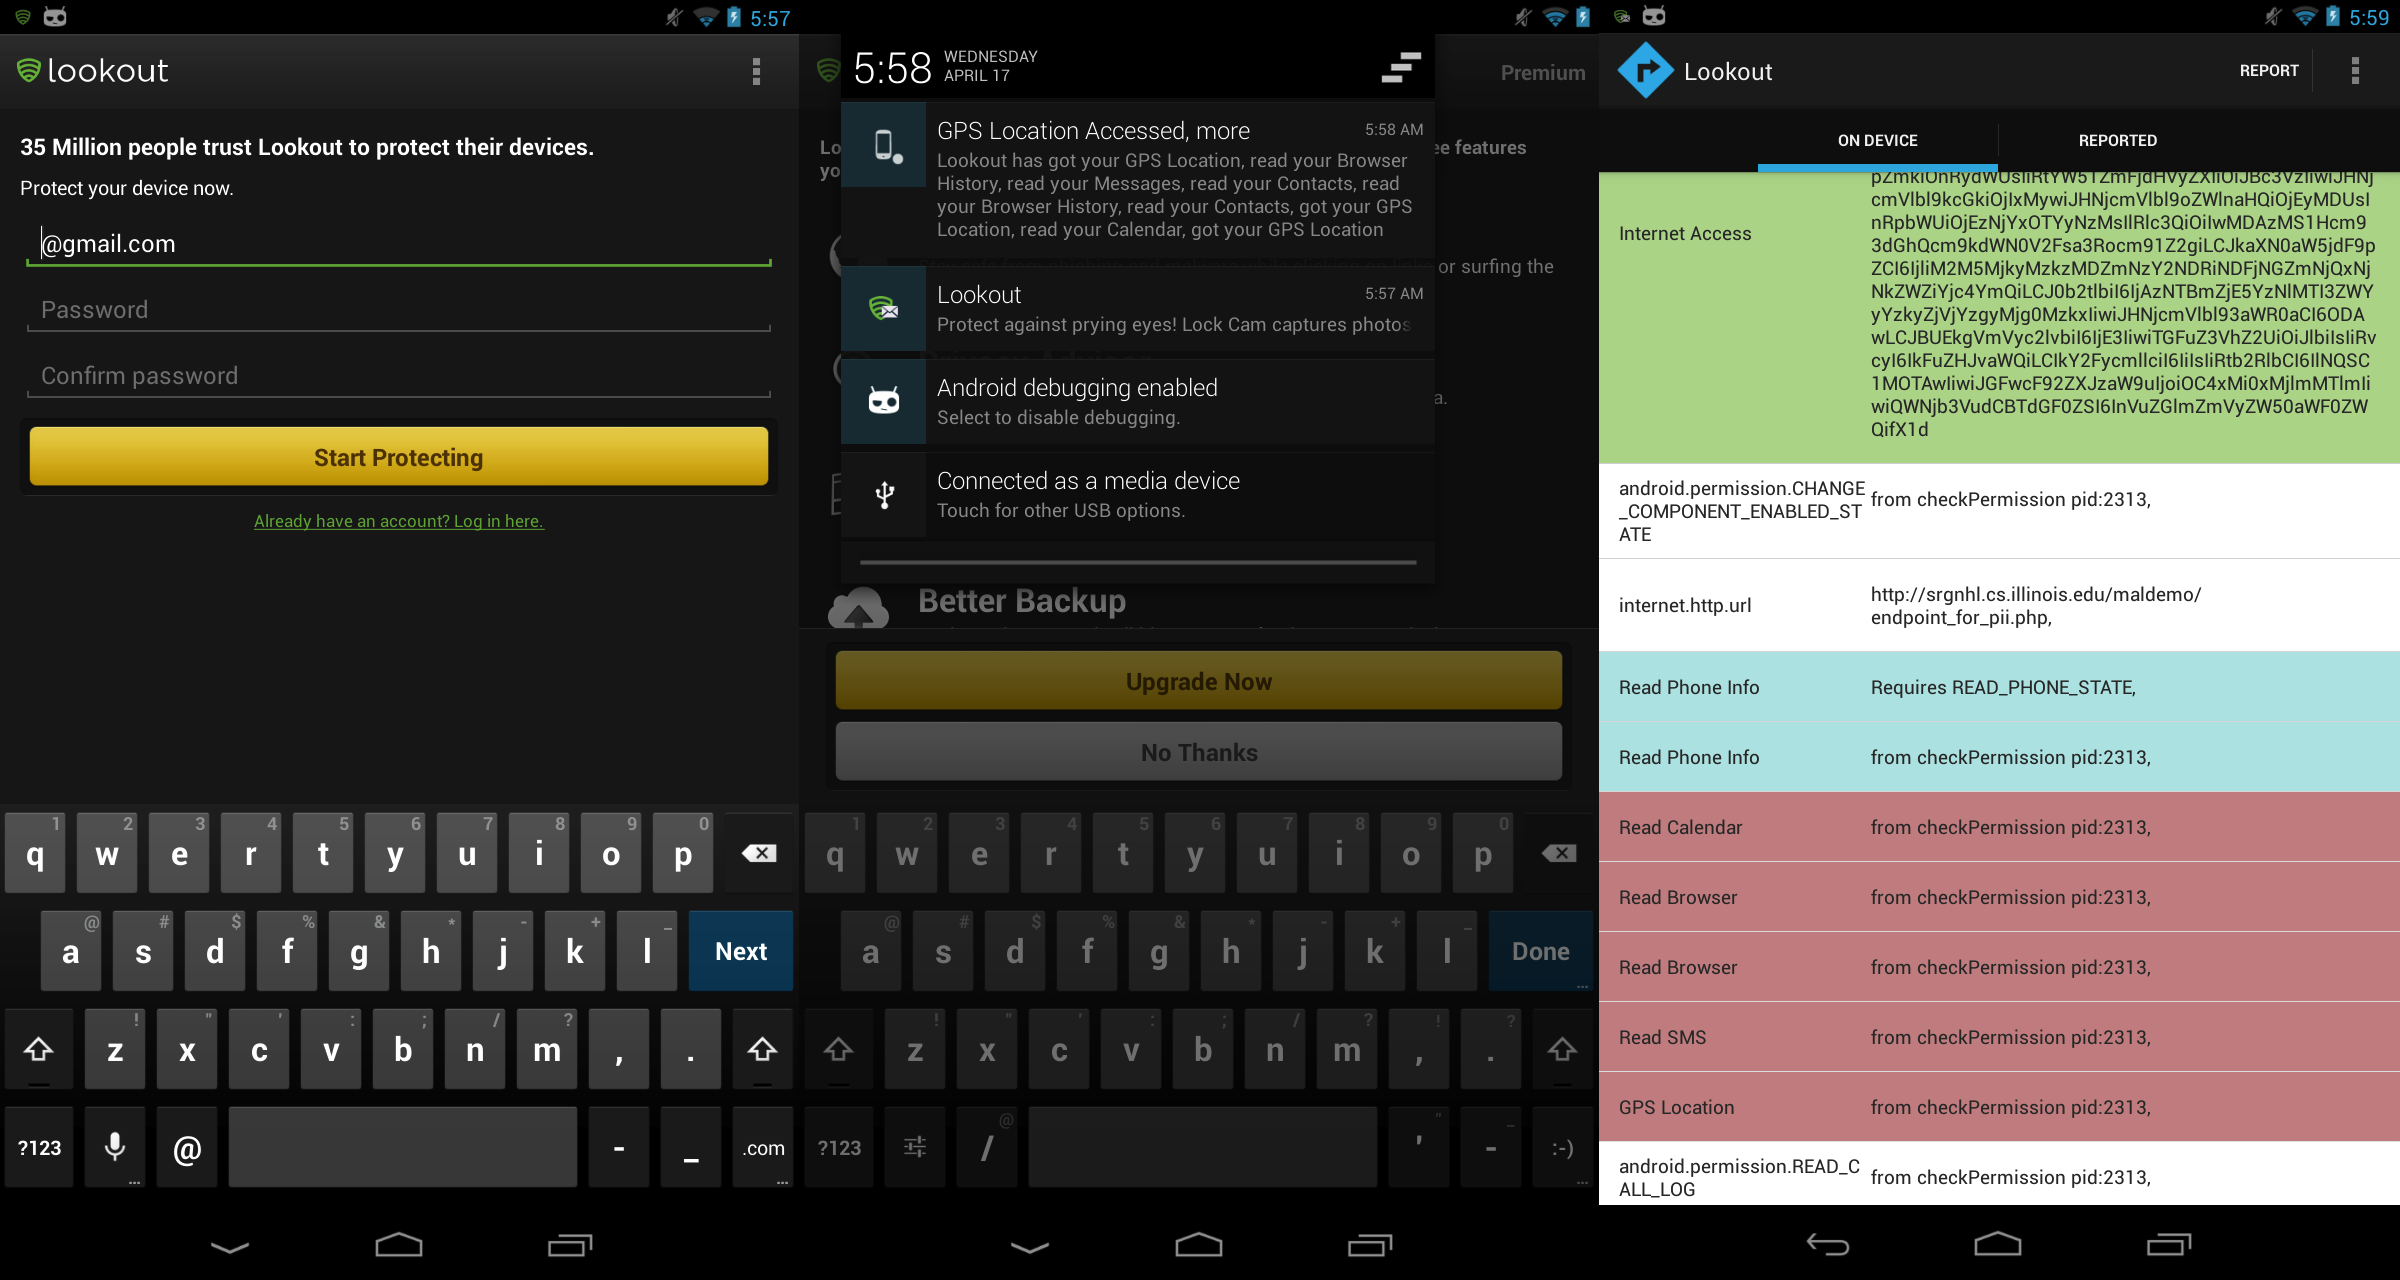
\includegraphics[width=1.0\columnwidth]{figs/lookout_detection}
\caption{AndroMEDA detecting the Info Theft IncognitoWare embedded within a security app }
\label{fig:infotheft_visual}
\end{center}
\end{figure}

\begin{figure}[h]
\begin{center}
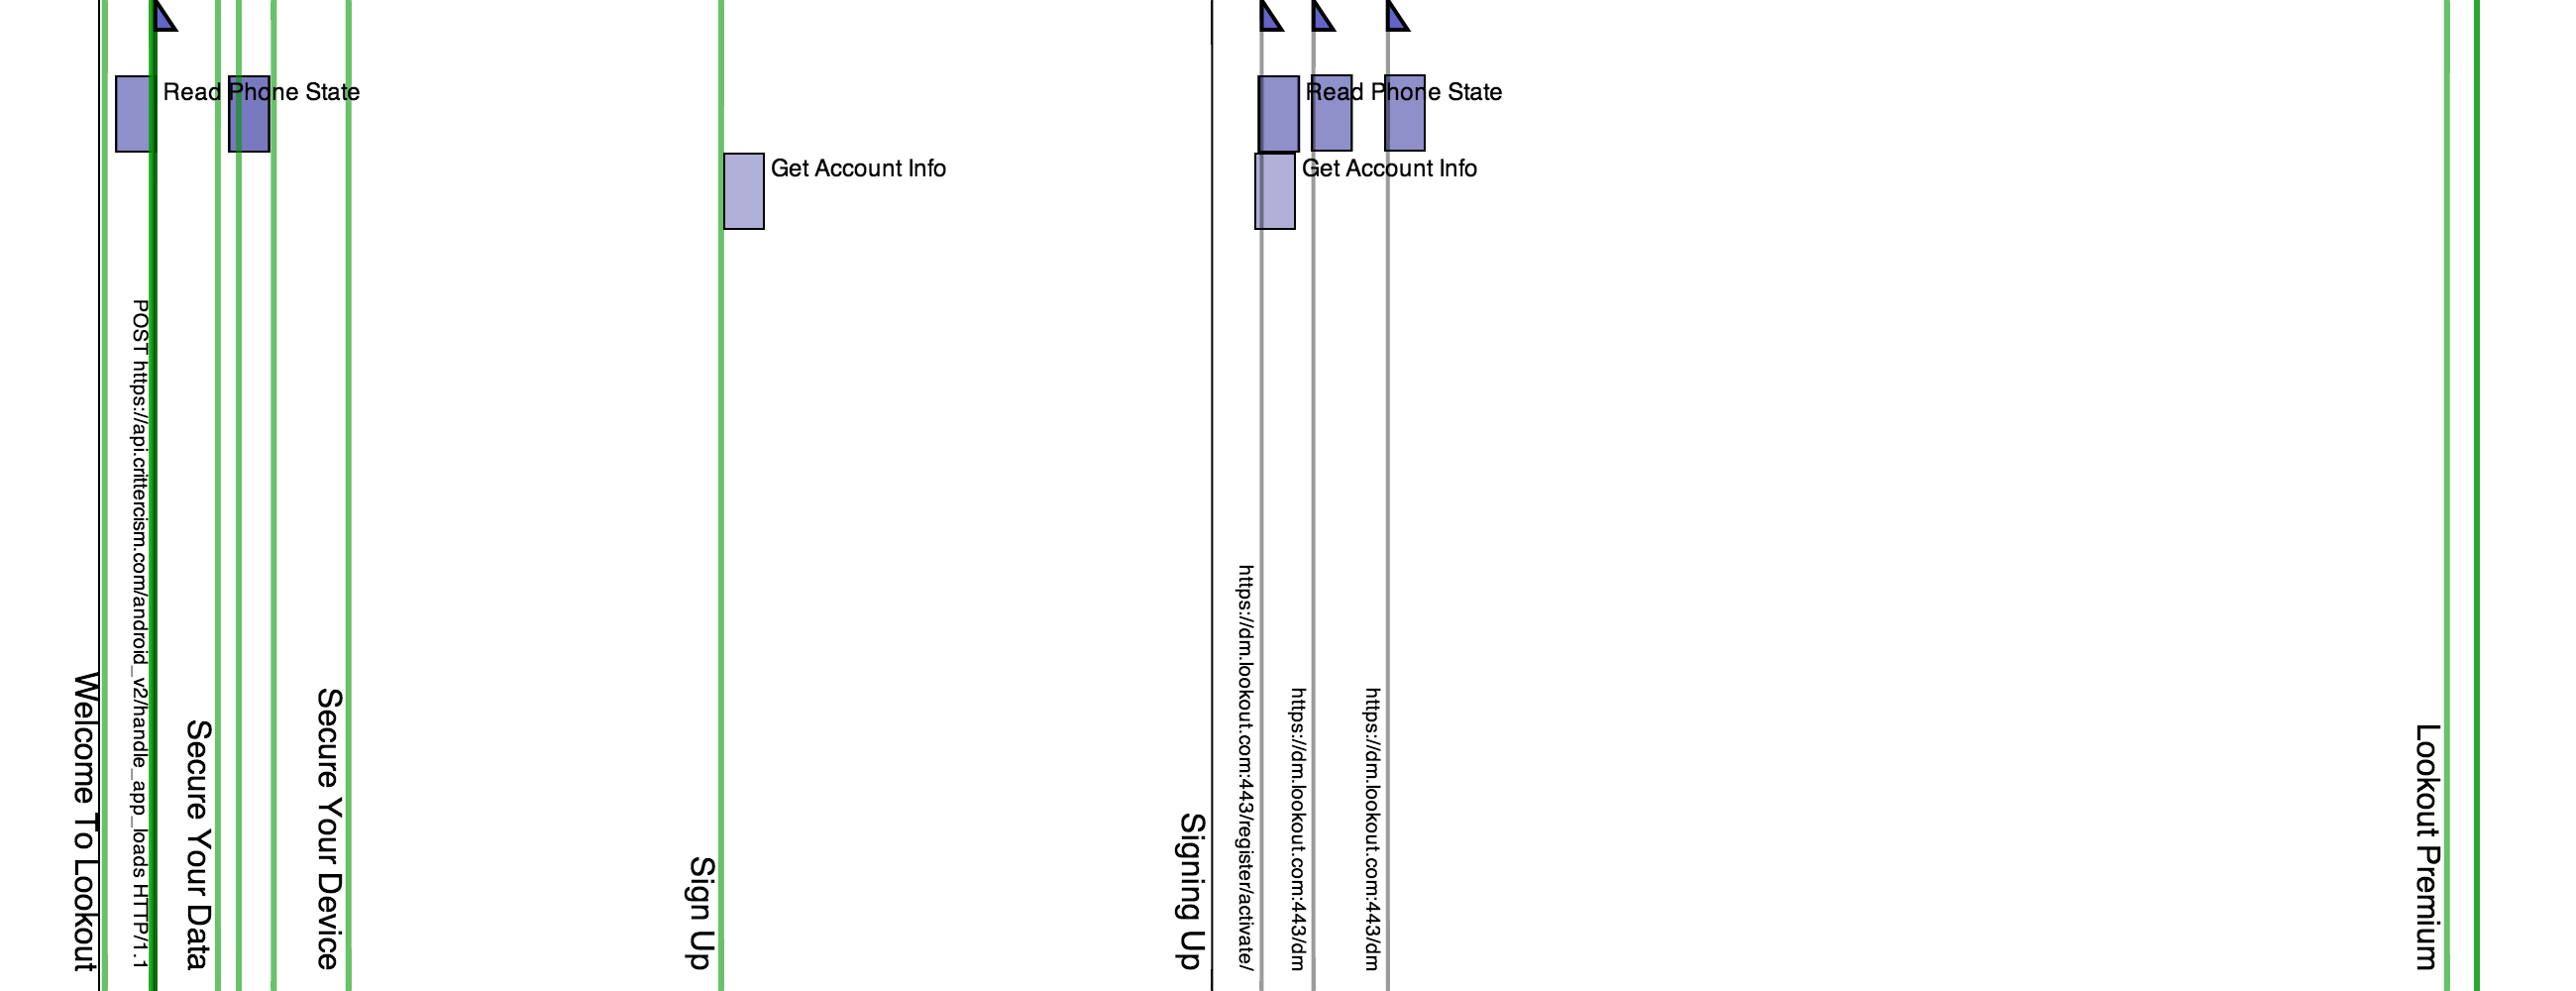
\includegraphics[width=1.0\columnwidth]{figs/AndroMEDA_Lookout_Notmalware}
\caption{AndroMEDA logs of the normal version of the security app }
\label{fig:infotheft_logs_nonmalware}
\end{center}
\end{figure}

\begin{figure}[h]
\begin{center}
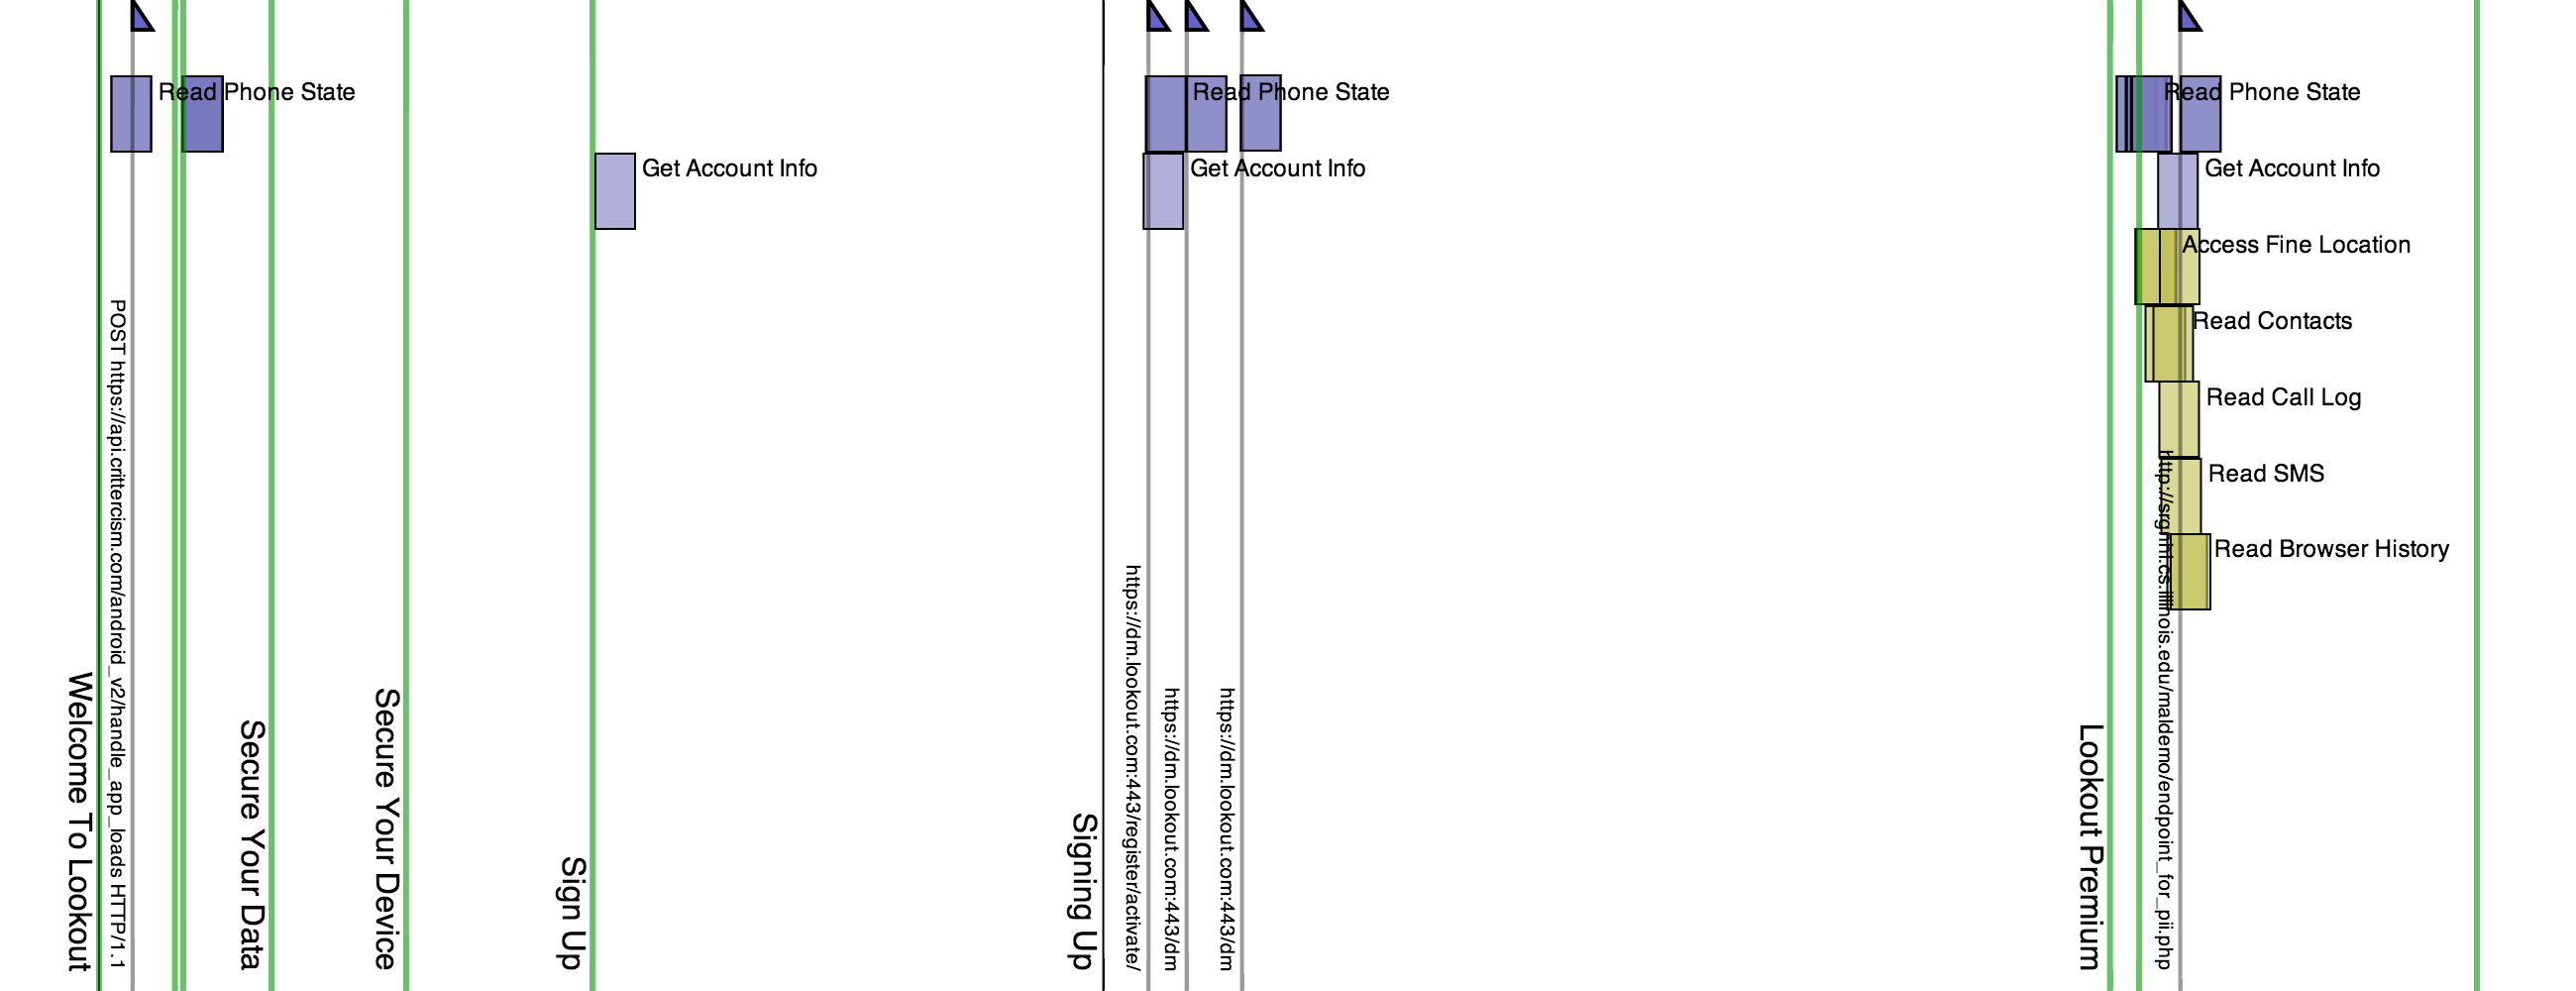
\includegraphics[width=1.0\columnwidth]{figs/AndroMEDA_Lookout_Malware}
\caption{AndroMEDA logs of Info Theft IncognitoWare embedded within a security app }
\label{fig:infotheft_logs_malware}
\end{center}
\end{figure}




\section{Spyware IncognitoWare}
Our next example of sophisticated IncognitoWare is designed to continuously spy on the user, while staying within the capabilities of a trusted app. We first find an app that has all the requirements for spyware: access to location, internet, wake lock, and starting at boot. We then introduce our malware, which is triggered an arbitrary amount of minutes after the first startup - 5 minutes is long enough to evade Google Bouncer\citep{mansfield2012android}. After that, the device wakes up every 5 minutes, gathers a location fix, and sends that information to a remote location. As before, many examples exist of apps that use similar behavior for non malicious purposes, making policies to guard against it difficult.

Once again, AndroMEDA can alert the user of this kind of behavior easily. Figure \ref{fig:spyware_visual} shows the user installing the app, starting it up, going to the home screen, and eventually noticing the suspicious behavior when the phone is idling. The user then inspects the logs for this app, Figure \ref{fig:spyware_logs_malware} (with context added), finds this to be a continuous occurrence, and decides that the app is malware. Compared with Figure \ref{fig:spyware_logs_nonmalware_noloc}, the app is clearly accessing location in a suspicious pattern, and the usage pattern is the key indicator. However, when compared to Figure \ref{fig:spyware_logs_nonmalware_location}, the main indicator is the address the information is going towards - an address not associated with the main app. The normal logs in Figure \ref{fig:spyware_logs_nonmalware_location} may break UAA for some users - the app logs the user's location in the background and sends it to a remote server. Overall, this highlights the ability of AndroMEDA to capture both the context and use of permissions - the patterns of access provide context, and the network locations provide use.




\begin{figure}[h]
\begin{center}
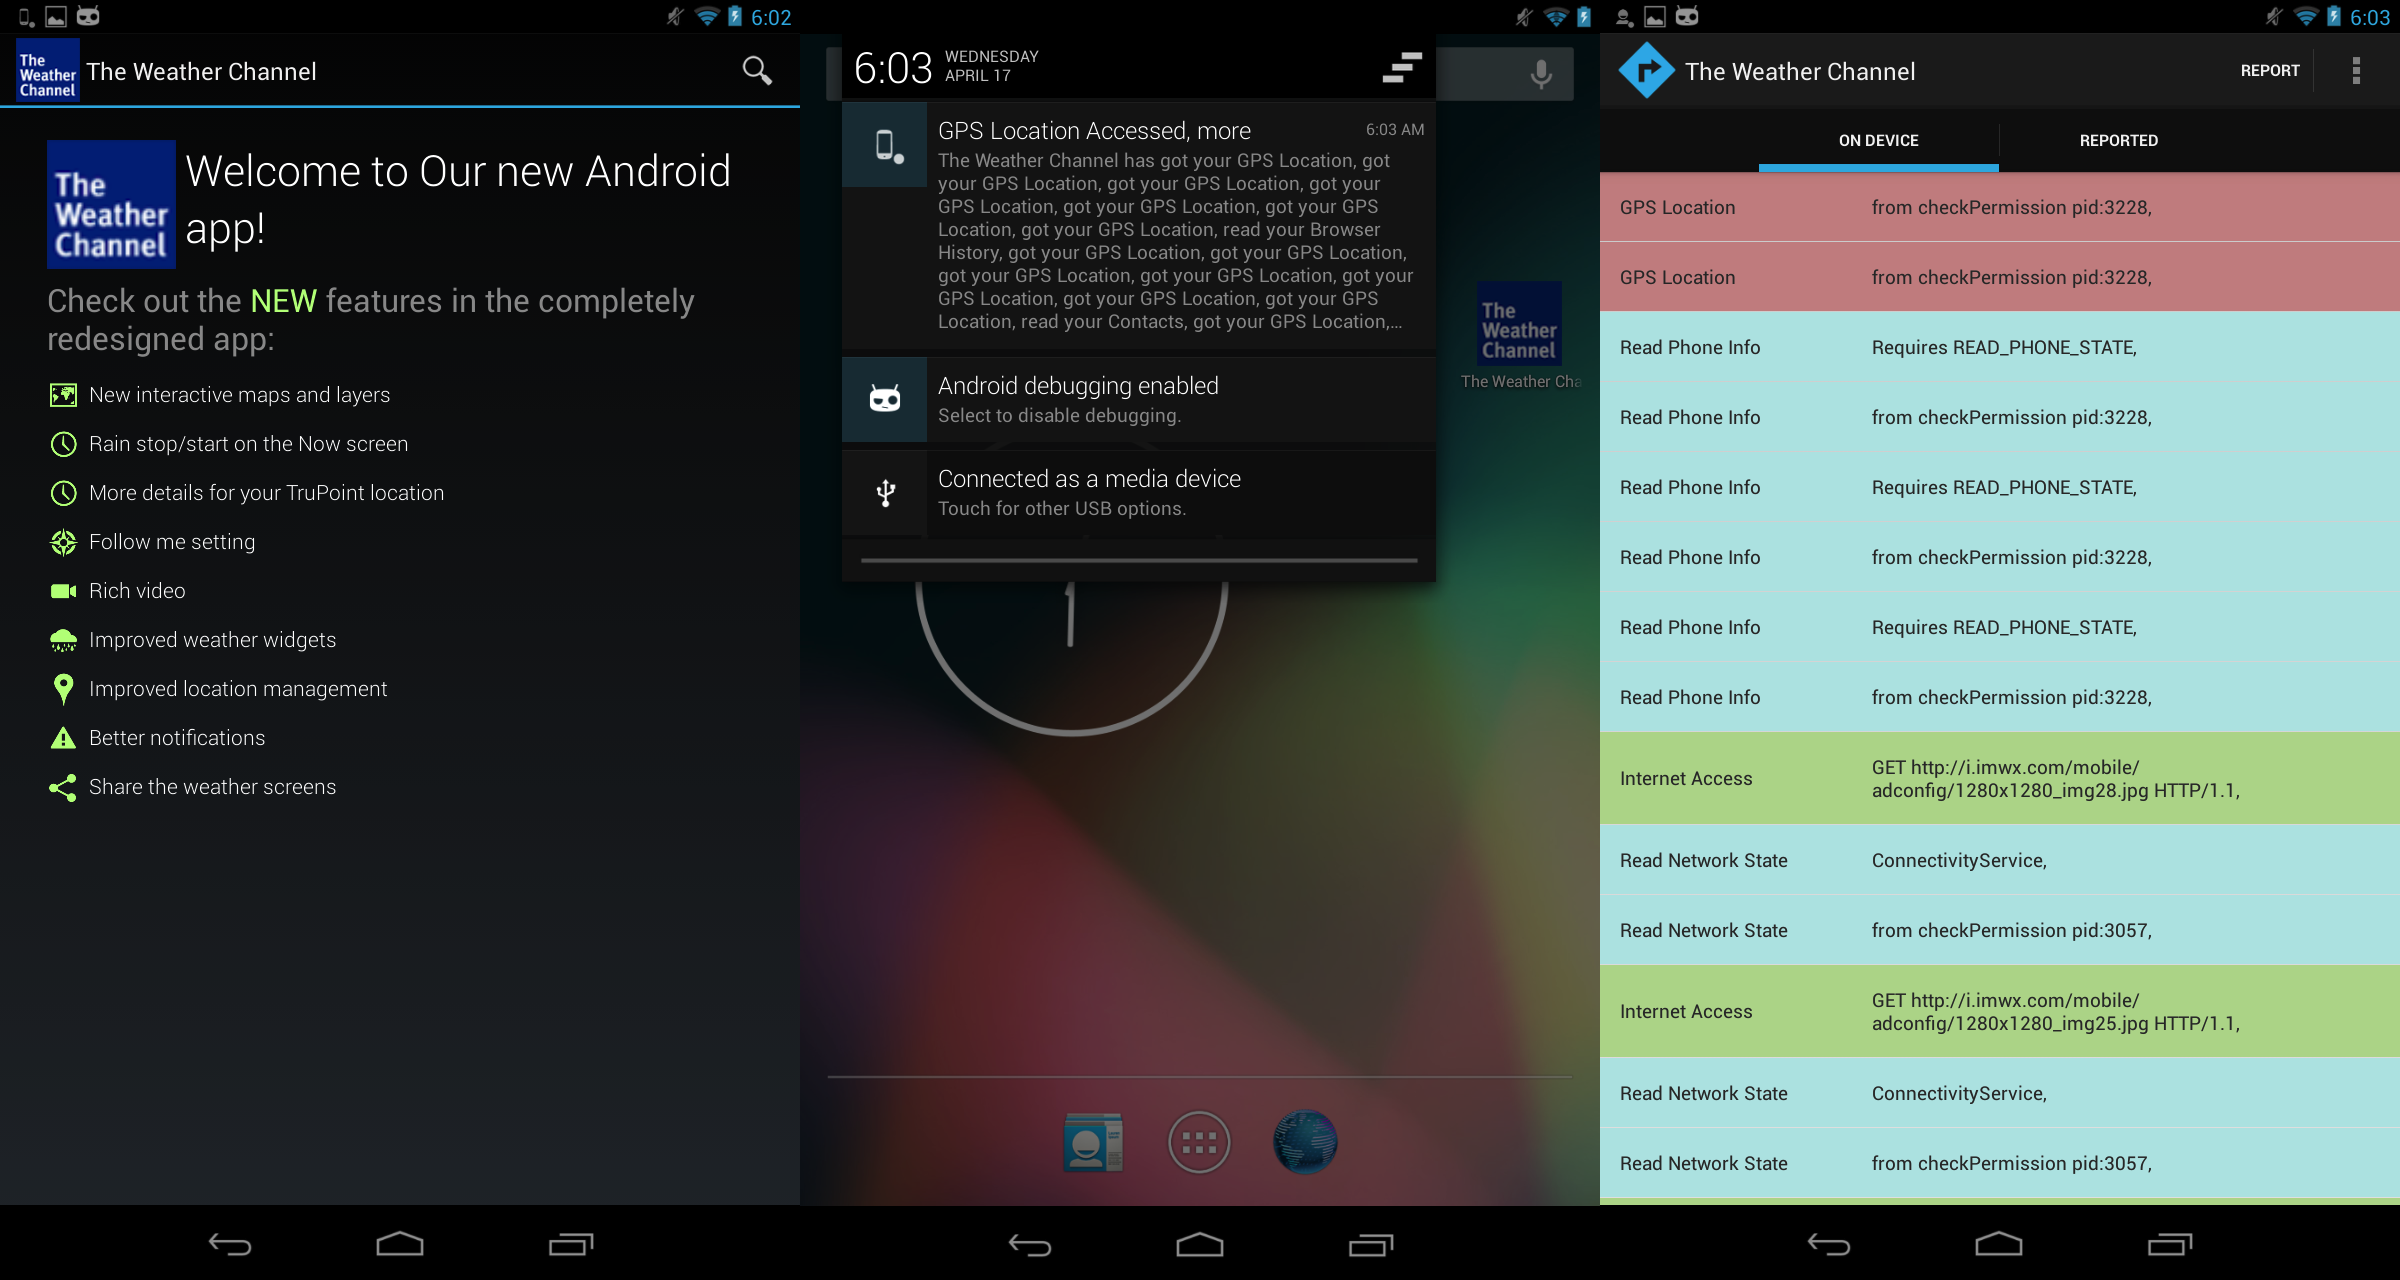
\includegraphics[width=1.0\columnwidth]{figs/weather_detection}
\caption{AndroMEDA detecting the Spyware IncognitoWare embedded within a weather app }
\label{fig:spyware_visual}
\end{center}
\end{figure}


\begin{figure}[h]
\begin{center}
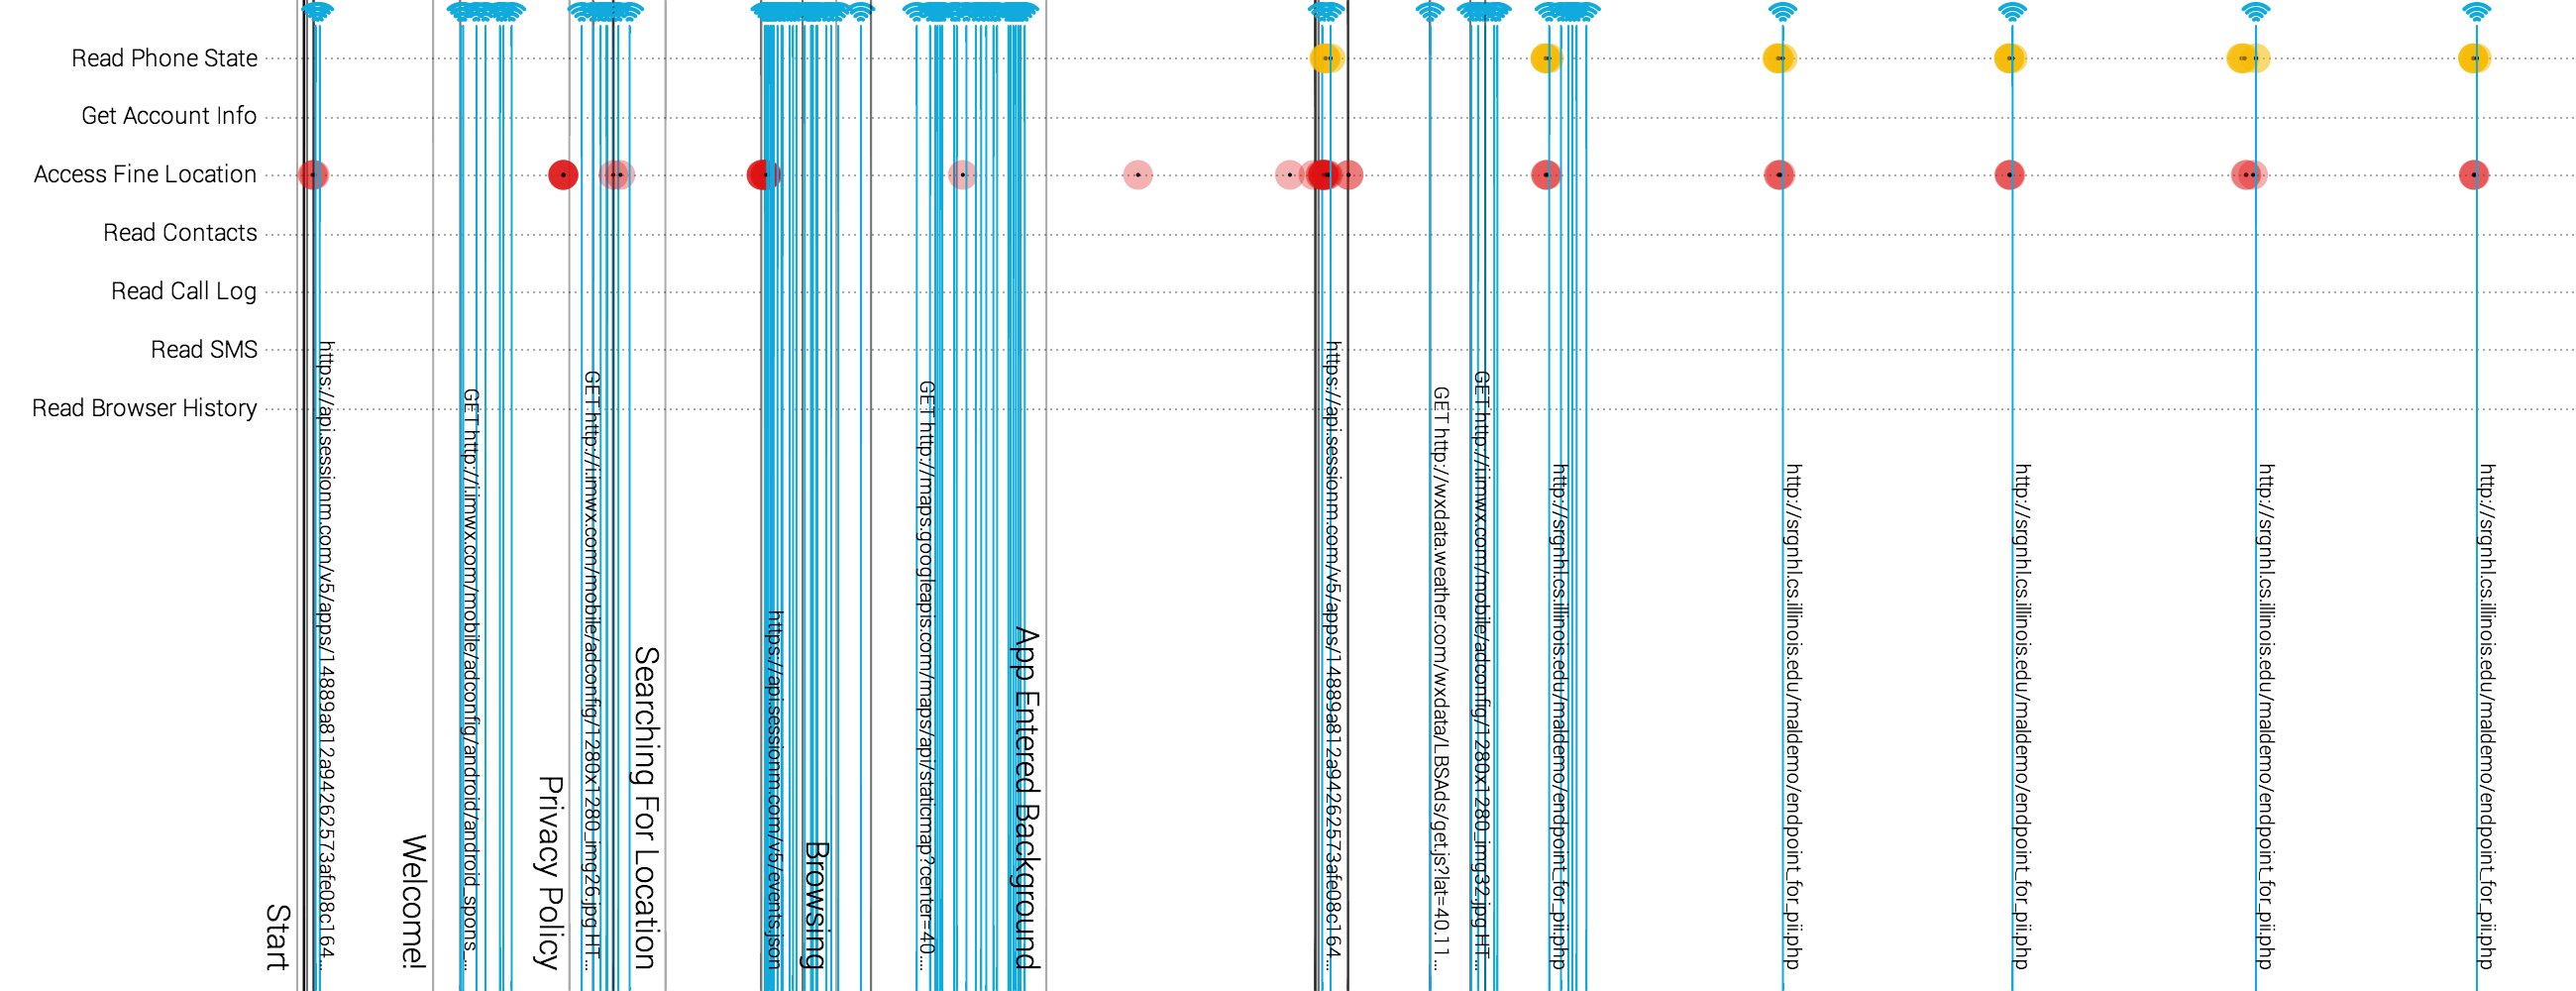
\includegraphics[width=1.0\columnwidth]{figs/AndroMEDA_Weather_Malware}
\caption{AndroMEDA logs of Spyware IncognitoWare embedded within a weather app }
\label{fig:spyware_logs_malware}
\end{center}
\end{figure}

\begin{figure}[h]
\begin{center}
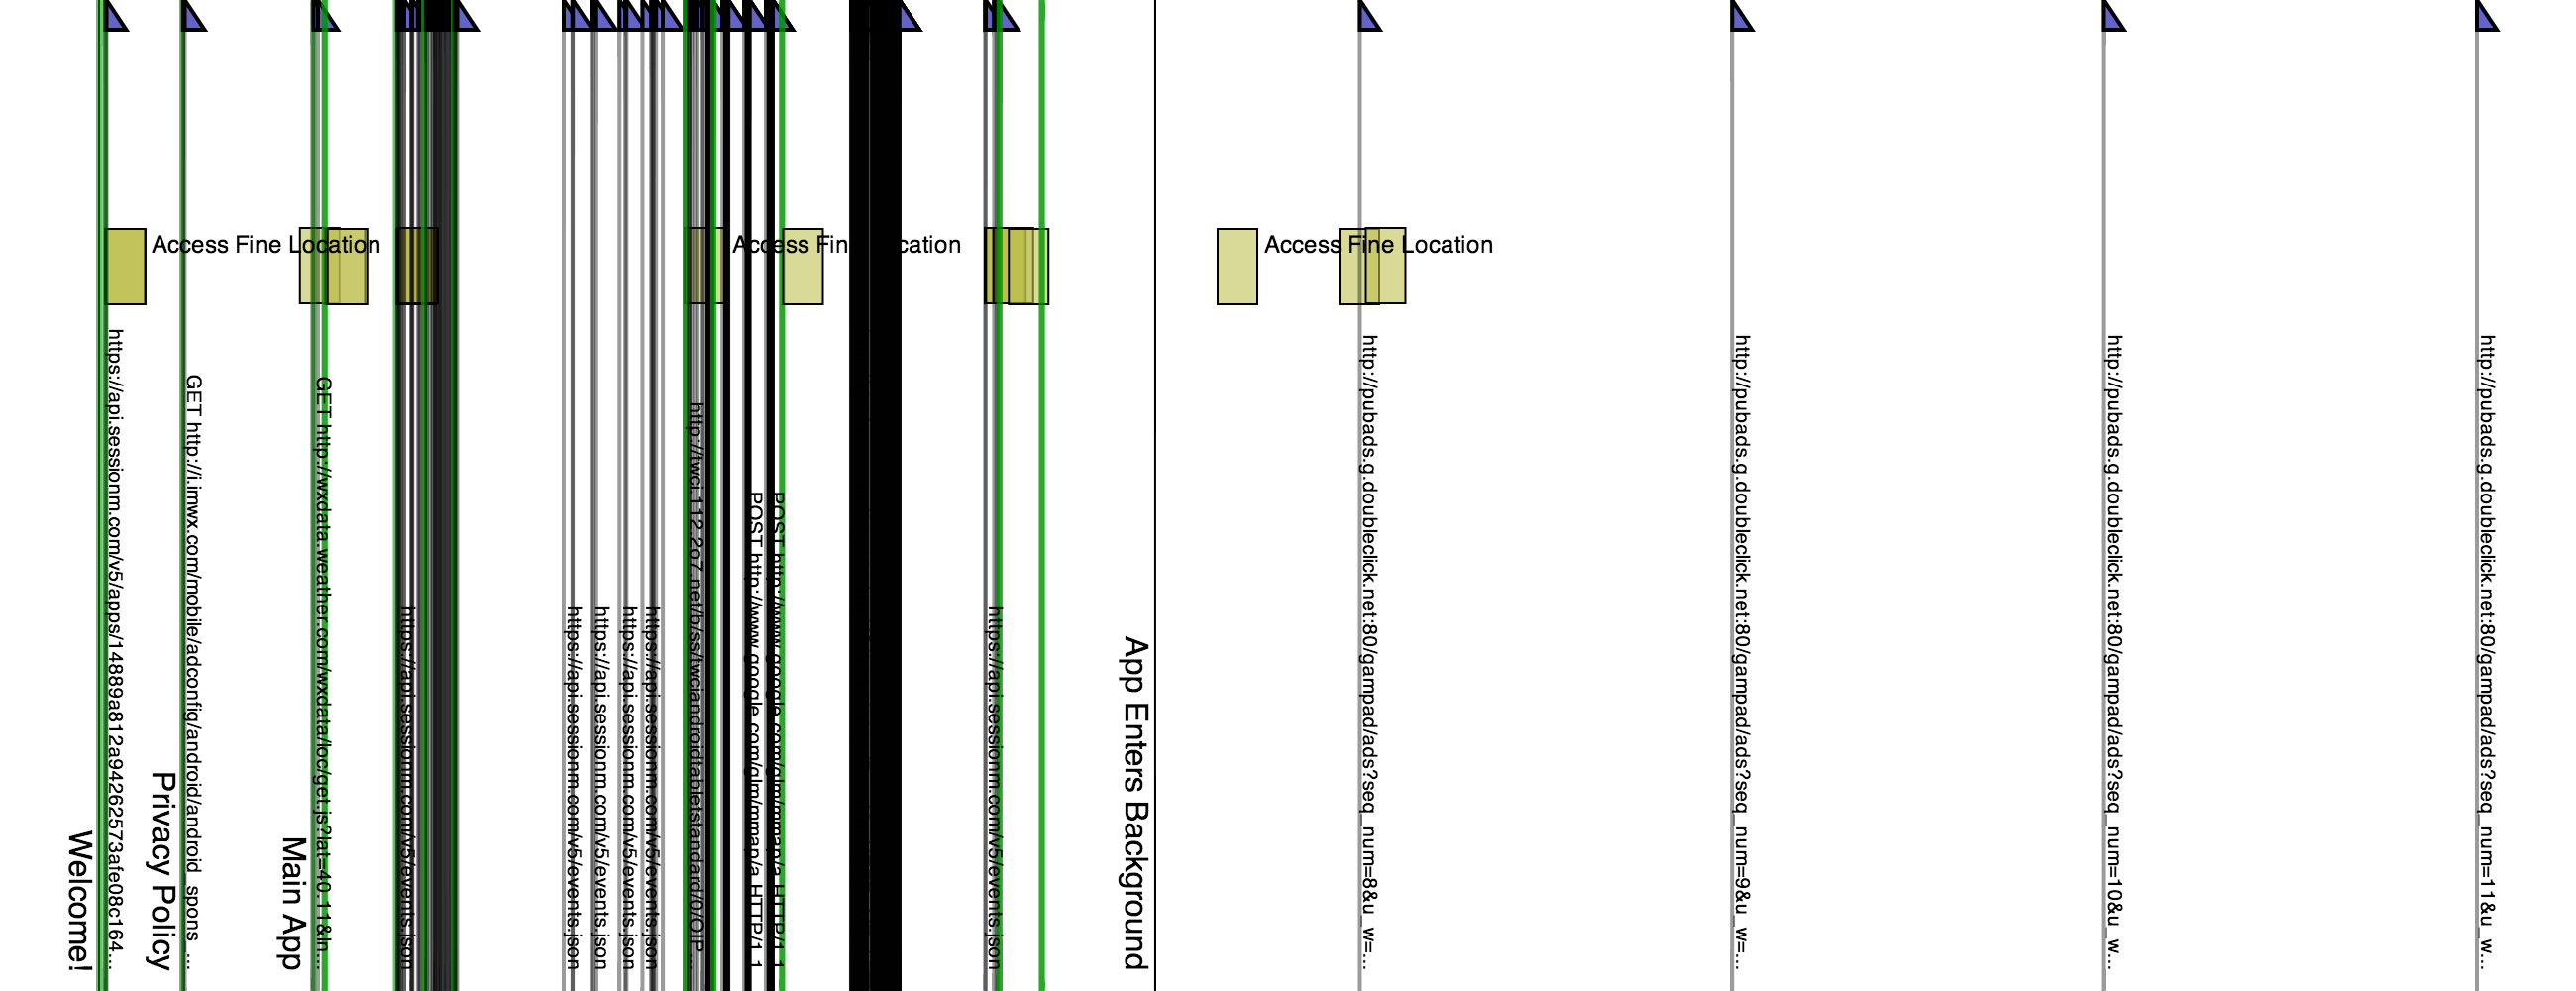
\includegraphics[width=1.0\columnwidth]{figs/AndroMEDA_Weather_Notmalware_Location}
\caption{AndroMEDA logs of a normal version of a weather app, when the user has consented to location gathering }
\label{fig:spyware_logs_nonmalware_location}
\end{center}
\end{figure}


\begin{figure}[h]
\begin{center}
\includegraphics[width=1.0\columnwidth]{figs/AndroMEDA_Weather_Notmalware_Nolocation}
\caption{AndroMEDA logs of a normal version of a weather app, when the user has not consented to location gathering }
\label{fig:spyware_logs_nonmalware_noloc}
\end{center}
\end{figure}


\section{Companion App}
When the user reviews the logs, they have the option to report suspicious behavior, giving a description of what the user was doing, and what the suspicious behavior was. These reports are collected in a centralized database. The companion app also listens for when the user installs new applications, and checks the same database to see if there are any existing reports. If the number of reports passes a threshold, the companion app will notify the user, giving them the ability to review what other people have reported about the apps. These features - being notified of suspicious apps and reviewing them - does not require the AndroMEDA extensions, and can be installed on any Android device. This enables a small set of users to alert a much larger population.

\section{Conclusion}
Overall, we have demonstrated that the ability to log and visualize app behavior can lead to an increased ability to detect malware. Our logs and visualizations show clear differences between actions that fall within the User-App Agreement, and actions that do not, even being able to visualize actions that may break some user's UAA but not others. Being able to report when an app breaks the UAA, and having that report spread to other users, enables AndroMEDA to become a community effort, further increasing its effectiveness.





